\clearpage
\item \subquestionpoints{10} \textbf{Coding problem.}
We will now consider the following dataset (the
formatting matches that of Datasets 1-4, except $x^{(i)}$ is 1-dimensional):
\begin{center}
	\url{data/ds5_{train,valid,test}.csv}	
\end{center}
In \texttt{src/p05b\_lwr.py}, implement locally weighted linear regression
using the normal equations you derived in Part (a) and using
%
\begin{equation*}
	w^{(i)} = \exp\left(-\frac{\|x^{(i)} - x\|_2^2}{2\tau^2}\right).
\end{equation*}
%
Train your model on the \texttt{train} split using $\tau = 0.5$, then run your
model on the \texttt{valid} split and report the mean squared error (MSE).
Finally plot your model's predictions on the validation set (plot the
training set with blue `x' markers and the validation set with a red `o'
markers). Does the model seem to be under- or overfitting?

\ifnum\solutions=1 {
  \begin{answer}

\begin{figure}[htbp]
    \centering
    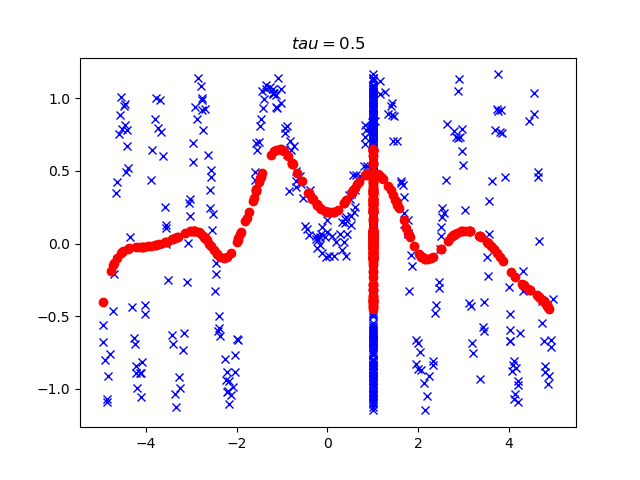
\includegraphics[width=0.5\linewidth]{pics/tau_0d5.png}
    \caption{tau=0.5}
\end{figure}

Final MSE is $0.33$. The model seems to underfitting.

\end{answer}

} \fi
